\documentclass[12pt]{article}

\usepackage{graphicx}  % Para incluir imagens
\usepackage{amsmath}   % Para usar matemática
\usepackage{hyperref}  % Para links

\title{Relatório de Experimento: Conexão de Máquinas e Teste de Ping no Cisco Packet Tracer}
\author{Alana Silva Barbosa}
\date{\today}

\begin{document}

\maketitle

\begin{abstract}
Este relatório descreve o experimento realizado no Cisco Packet Tracer, no qual foram conectadas duas máquinas através de um cabo Coper Cross-Over, e foi feito um teste de comunicação entre elas utilizando o comando \texttt{ping}. O objetivo foi verificar a conectividade entre as duas máquinas e realizar o envio de pacotes de dados.
\end{abstract}

\section{Introdução}

O Cisco Packet Tracer é uma ferramenta de simulação de redes amplamente utilizada no ensino de redes de computadores. Este experimento tem como objetivo a criação de uma rede simples, conectando duas máquinas através de um cabo cross e verificando a comunicação entre elas usando o comando \texttt{ping}. Este tipo de teste é fundamental para diagnosticar problemas de conectividade e entender o funcionamento da rede.

\section{Materiais e Métodos}

Para a realização do experimento, os seguintes componentes foram utilizados:
\begin{itemize}
    \item Cisco Packet Tracer;
    \item 2 Computadores (PC-PT);
    \item 1 Cabo Cross-over;
    \item Endereços IP e máscara subrede configurados manualmente.
\end{itemize}

O procedimento seguido foi:
\begin{enumerate}
    \item Iniciar o Cisco Packet Tracer e criar um novo projeto;
    \item Adicionar duas máquinas (PC0 e PC1) ao projeto;
    \item Conectar as máquinas utilizando um cabo cross-over entre as portas de rede das duas máquinas;
    \item Configurar os endereços IP das máquinas. A máquina PC0 recebeu o IP \texttt{192.168.10.1}, e a máquina PC1 recebeu o IP \texttt{192.168.10.2/24};
    \item Verificar a conectividade utilizando o comando \texttt{ping} a partir da máquina PC0 para a máquina PC1.
\end{enumerate}

\section{Resultados}

Após a configuração da rede e a execução do comando \texttt{ping}, a máquina PC0 enviou pacotes para a máquina PC1. O teste foi bem-sucedido, e os pacotes foram recebidos pela máquina PC1, confirmando que a comunicação entre as duas máquinas estava estabelecida.

\begin{figure}[h!]
    \centering
    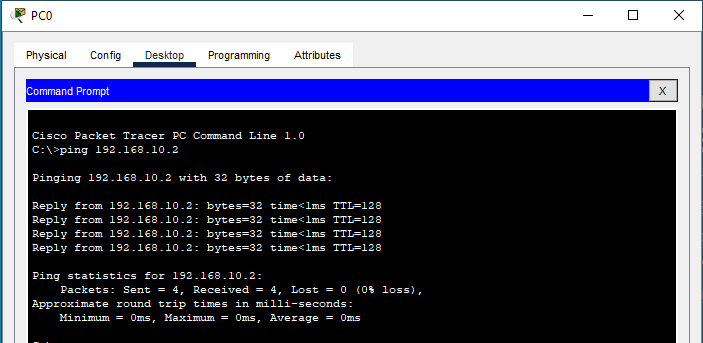
\includegraphics[width=0.7\textwidth]{teste_ping.png}
    \caption{Resultado do comando \texttt{ping} da máquina PC0 para a máquina PC1}
    \label{fig:teste_ping}
\end{figure}

A Figura \ref{fig:ping_output} mostra o resultado do comando \texttt{ping} realizado na máquina PC0, indicando que os pacotes foram enviados e recebidos com sucesso, não houve perda de pacotes.

\begin{figure}[h!]
    \centering
    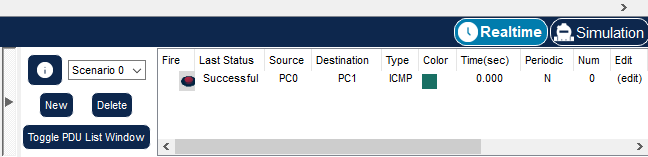
\includegraphics[width=0.7\textwidth]{teste_ICMP.png}
    \caption{Resultado do envio de pacotes da máquina PC0 para a máquina PC1}
    \label{fig:teste_ICMP}
\end{figure}

A Figura \ref{fig:teste_ICMP} mostra o resultado do envio de pacotes ICMP realizado, indicando que os pacotes foram enviados e recebidos com sucesso, não houve perda de pacotes.

\section{Discussão}

O experimento demonstrou que a comunicação entre as duas máquinas foi bem-sucedida, e os pacotes de dados foram trocados sem qualquer empecilho. A utilização de um cabo cross-over foi crucial para conectar diretamente as duas máquinas, não havendo necessidade de uso de um switch ou roteador que realizasse a intermediação entre as máquinas.

Este tipo de configuração apesar de simples, se mostra útil em cenários onde é necessário testar a conectividade entre dois dispositivos diretamente. A ferramenta Cisco Packet Tracer se mostrou eficiente para simular essa rede e realizar os testes de conectividade propostos.

\section{Conclusão}

O experimento foi concluído com sucesso, confirmando a conectividade entre as duas máquinas. A configuração de rede utilizando o cabo cross-over e a definição de endereços IP foram fundamentais para o sucesso do experimento.

Futuros experimentos podem explorar a utilização de outros tipos de cabos, como o cabo direto, e a adição de dispositivos intermediários, como switches e roteadores, para ampliar a rede e testar a conectividade em cenários mais complexos.

\section{Referências}
\begin{itemize}
    \item Material eleborado pelo professor Macêdo Firmino (IFRS) e disponibilizado na plataforma CANVAS pelo professor Leonardo de Mélo João(PUCMG)
\end{itemize}

\end{document}
